\par Se desea determinar si la pantalla diseñada cumple con el requerimiento de pertenecer a la Categoría B3 de la norma UNE-EN 1793-2:2014, Anexo A. Para ello se coloca una muestra de de $10 m^2$ entre las cámaras de transmisión horizontal del LAL y se miden, a tercios de octavas entre las frecuencias  100Hz y 5000Hz, los niveles de presión sonora en cada cámara, el ruido de fondo y los tiempos de reverberación. Dichas mediciones se realizan respetando el procedimiento propuesto por la Norma IRAM 4063-3/2002: Acústica. Medición en laboratorio del aislamiento acústico a ruido aéreo de los elementos de construcción; e IRAM 4063-1/2002.

\par A partir de las mediciones realizadas se obtuvieron los datos presentados en la Tabla~\tableref{tab:Niveles_sonoros_y_tiempos_de_reverberacion_medidos}.

\begin{table}[H]
    \centering
    \begin{tabular}{|c|c|c|c|c|} \hline
        \textbf{Banda} & \textbf{L1 (dB)} & \textbf{L2 (dB)} & \textbf{RF (dB)} & \textbf{TR (s)} \\ \hline \hline
        50& 62,5&	52,9&	17,9&	6,910 \\ \hline
        63& 62,6&	51,3&	19,5&	7,780 \\ \hline
        80& 76,5&	61,4&	23,4&	7,320 \\ \hline
        100& 80,0&	66,6&	34,7&	5,970 \\ \hline
        125& 81,2&  68,6&	27,4&	5,300 \\ \hline
        160& 80,6&	64,4&	19,6&	3,690\\ \hline
        200& 77,9&	59,4&	9,2 &	2,950 \\ \hline
        250& 79,1&	56,0&	6,5 &	2,080\\ \hline
        315& 79,6&	52,7&	5,8 &	2,210 \\ \hline
        400& 82,8&	52,1&	4,5 &	1,880 \\ \hline
        500& 81,8&	47,9&	3,8 &	1,880 \\ \hline
        630& 78,2&	44,2&	5,3 &	1,780 \\ \hline
        800& 77,7&	44,7&	5,1 &	1,800 \\ \hline
        1000& 79,0&	46,4&	5,1 &	1,770 \\ \hline
        1250& 78,1&	46,0&	9,7 &	1,730 \\ \hline
        1600& 79,9&	51,0&	7,5 &	1,830 \\ \hline
        2000& 79,8&	50,8&	7,1 &	1,840 \\ \hline
        2500& 79,4&	47,2&	6,4 &	1,780 \\ \hline
        3150& 79,1&	50,1&	6,9 &	1,810 \\ \hline
        4000& 82,3&	51,6&	7,8 &	1,640 \\ \hline
        5000& 80,7&	50,5&	8,0 &	1,480\\ \hline
    \end{tabular}
    \caption{Niveles sonoros y tiempos de reverberación medidos}
    \label{tab:Niveles_sonoros_y_tiempos_de_reverberacion_medidos}
\end{table}

\par El criterio de clasificación de la pantalla requiere el cálculo del Índice de evaluación del aislamiento acústico. Este mismo corresponde a la diferencia entre: la suma energética de niveles de presión sonora de cada tercio de octava ($L_i$), y la suma energética de la diferencia entre los niveles sonoros y el índice de reducción sonora ($L_i - R_i$).

$$
        DL_R  = 10 \cdot log \Big(\sum^{18}_{i=1} 10^{{L_i}/{10}} \Big) -10 \cdot log  \Big( \sum_{i=1}^{18} 10^{(L_i - R_i)/{10}} \Big) $$
    
$$
        = 10 \cdot log \Big(\sum^{18}_{i=1} 10^{{L_i}\cdot0.1} \Big) -10 \cdot log  \Big( \sum_{i=1}^{18} 10^{L_i\cdot0.1} \cdot 10^{-R_i\cdot0.1} \Big) $$
    
\begin{equation}
        DL_R = -10\cdot log \Big( \frac{\sum_{i=1}^{18} 10^{0.1 \cdot L_i} \cdot 10^{-0.1 \cdot R_i}}{\sum^{18}_{i=1} 10^{0.1 \cdot L_i} }\Big)
    \label{eq:DL_R}
\end{equation}

\par En donde:
\begin{itemize}
    \item $R_i$: Índice de reducción sonora en la i-ésima banda de tercio de octava correspondiente a la muestra ensayada.
    \item $L_i$: Nivel de presión sonora de ruido normalizado ponderado A, en dB, de la i-ésima banda de tercio de octava del ruido normalizado ferroviario (UNE-EN 16272-3).
\end{itemize}
    

\par Para obtener el resultado de dicha ecuación, necesitamos los valores de $R_i$ para cada tercio de octava. Estos valores se obtienen de la siguiente forma:
\begin{equation}
    R_i = L_1 - L_2 + 10 \cdot log \Big(\frac{S_{muestra}}{A_{iEq}}\Big)
    \label{eq:indice_reduccion_sonora}
\end{equation}

\par Donde:
\begin{itemize}
    \item $L_1$ y $L_2$: corresponden los niveles sonoros continuos equivalentes medidos en cámara emisora y receptora respectivamente, en dB.
    \item $S_{muestra}$: es la superficie real de la muestra ensayada, es decir, $10m^2$.
    \item $A_{iEq}$: área equivalente
\end{itemize}

\par Es necesario a continuación calcular el \textit{área equivalente} del material ensayado (Ecuación~\eqref{eq:aerea_equivalente}), correspondiente a la absorción de una superficie con coeficiente de absorción acústica igual a 1 y área igual a la absorción total del elemento. 

\begin{equation}
    A_{i Eq} =  \frac{55.3}{C} \cdot \frac{V_{Receptora}}{TR_i}
    \label{eq:aerea_equivalente}
\end{equation}

\par Donde:
\begin{itemize}
    \item $C$: es la velocidad del sonido en $\frac{m}{seg}$, la cuál se calcula considerando la temperatura de las cámaras durante el ensayo mediante $C = 332\cdot m/s+ 0.608 \cdot T^{\circ}$. Para $T= 20^{\circ}C$, $C = 344.16 m/seg$
    \item $V_{Receptora}$: Es el volúmen de la cámara receptora, que es $113,9m^3$
    \item $TR_i$: Es el tiempo de reverberación percibido en la cámara receptora en la i-ésima banda medida.
\end{itemize}

\par A partir de estas relaciones, logramos obtener los valores del Índice de Reducción Sonora ($R_i$) plasmados en la Tabla~\tableref{tab:reduccion_sonora_R}:

\begin{table}[H]
    \centering
    \begin{tabular}{|c|c|} \hline
        \textbf{Banda} & \textbf{R[dB]} \\\hline
        50 & 15,37\\\hline
        63 & 17,59\\\hline
        80 & 21,12 \\\hline
        100 & 18,54\\\hline
        125 & 17,22\\\hline
        160 & 19,25\\\hline
        200 & 20,57\\\hline
        250 & 23,66\\\hline
        315 & 27,72\\\hline
        400 & 30,82\\\hline
        500 & 34,02\\\hline
        630 & 33,88\\\hline
        800 & 32,93\\\hline
        1000& 32,46\\\hline
        1250& 31,86\\\hline
        1600& 28,90\\\hline
        2000& 29,02\\\hline
        2500& 32,08\\\hline
        3150& 28,95\\\hline
        4000& 30,22\\\hline
        5000& 29,28\\\hline
    \end{tabular}
    \caption{valores del Índice de Reducción Sonora R}
    \label{tab:reduccion_sonora_R}
\end{table}

\par A partir de los valores obtenidos, comenzamos el análisis de las mediciones realizadas. En primer lugar, sabemos que el instrumento de medición ubicado en la cámara receptora estará ligado a un ruido de fondo indicado en la tabla~\tableref{tab:Niveles_sonoros_y_tiempos_de_reverberacion_medidos}. Bajo esta consideración, presentamos un gráfico con los valores obtenidos. En el Gráfico~\figref{fig::comparacion_niveles_sonoros} podemos observar de forma simultánea, los niveles sonoros medidos en la cámara emisora y la cámara receptora, y el ruido de fondo de la sala cuando no se esta emitiendo la banda de sonido de prueba.

%\begin{figure}[H]
%	\centering
%	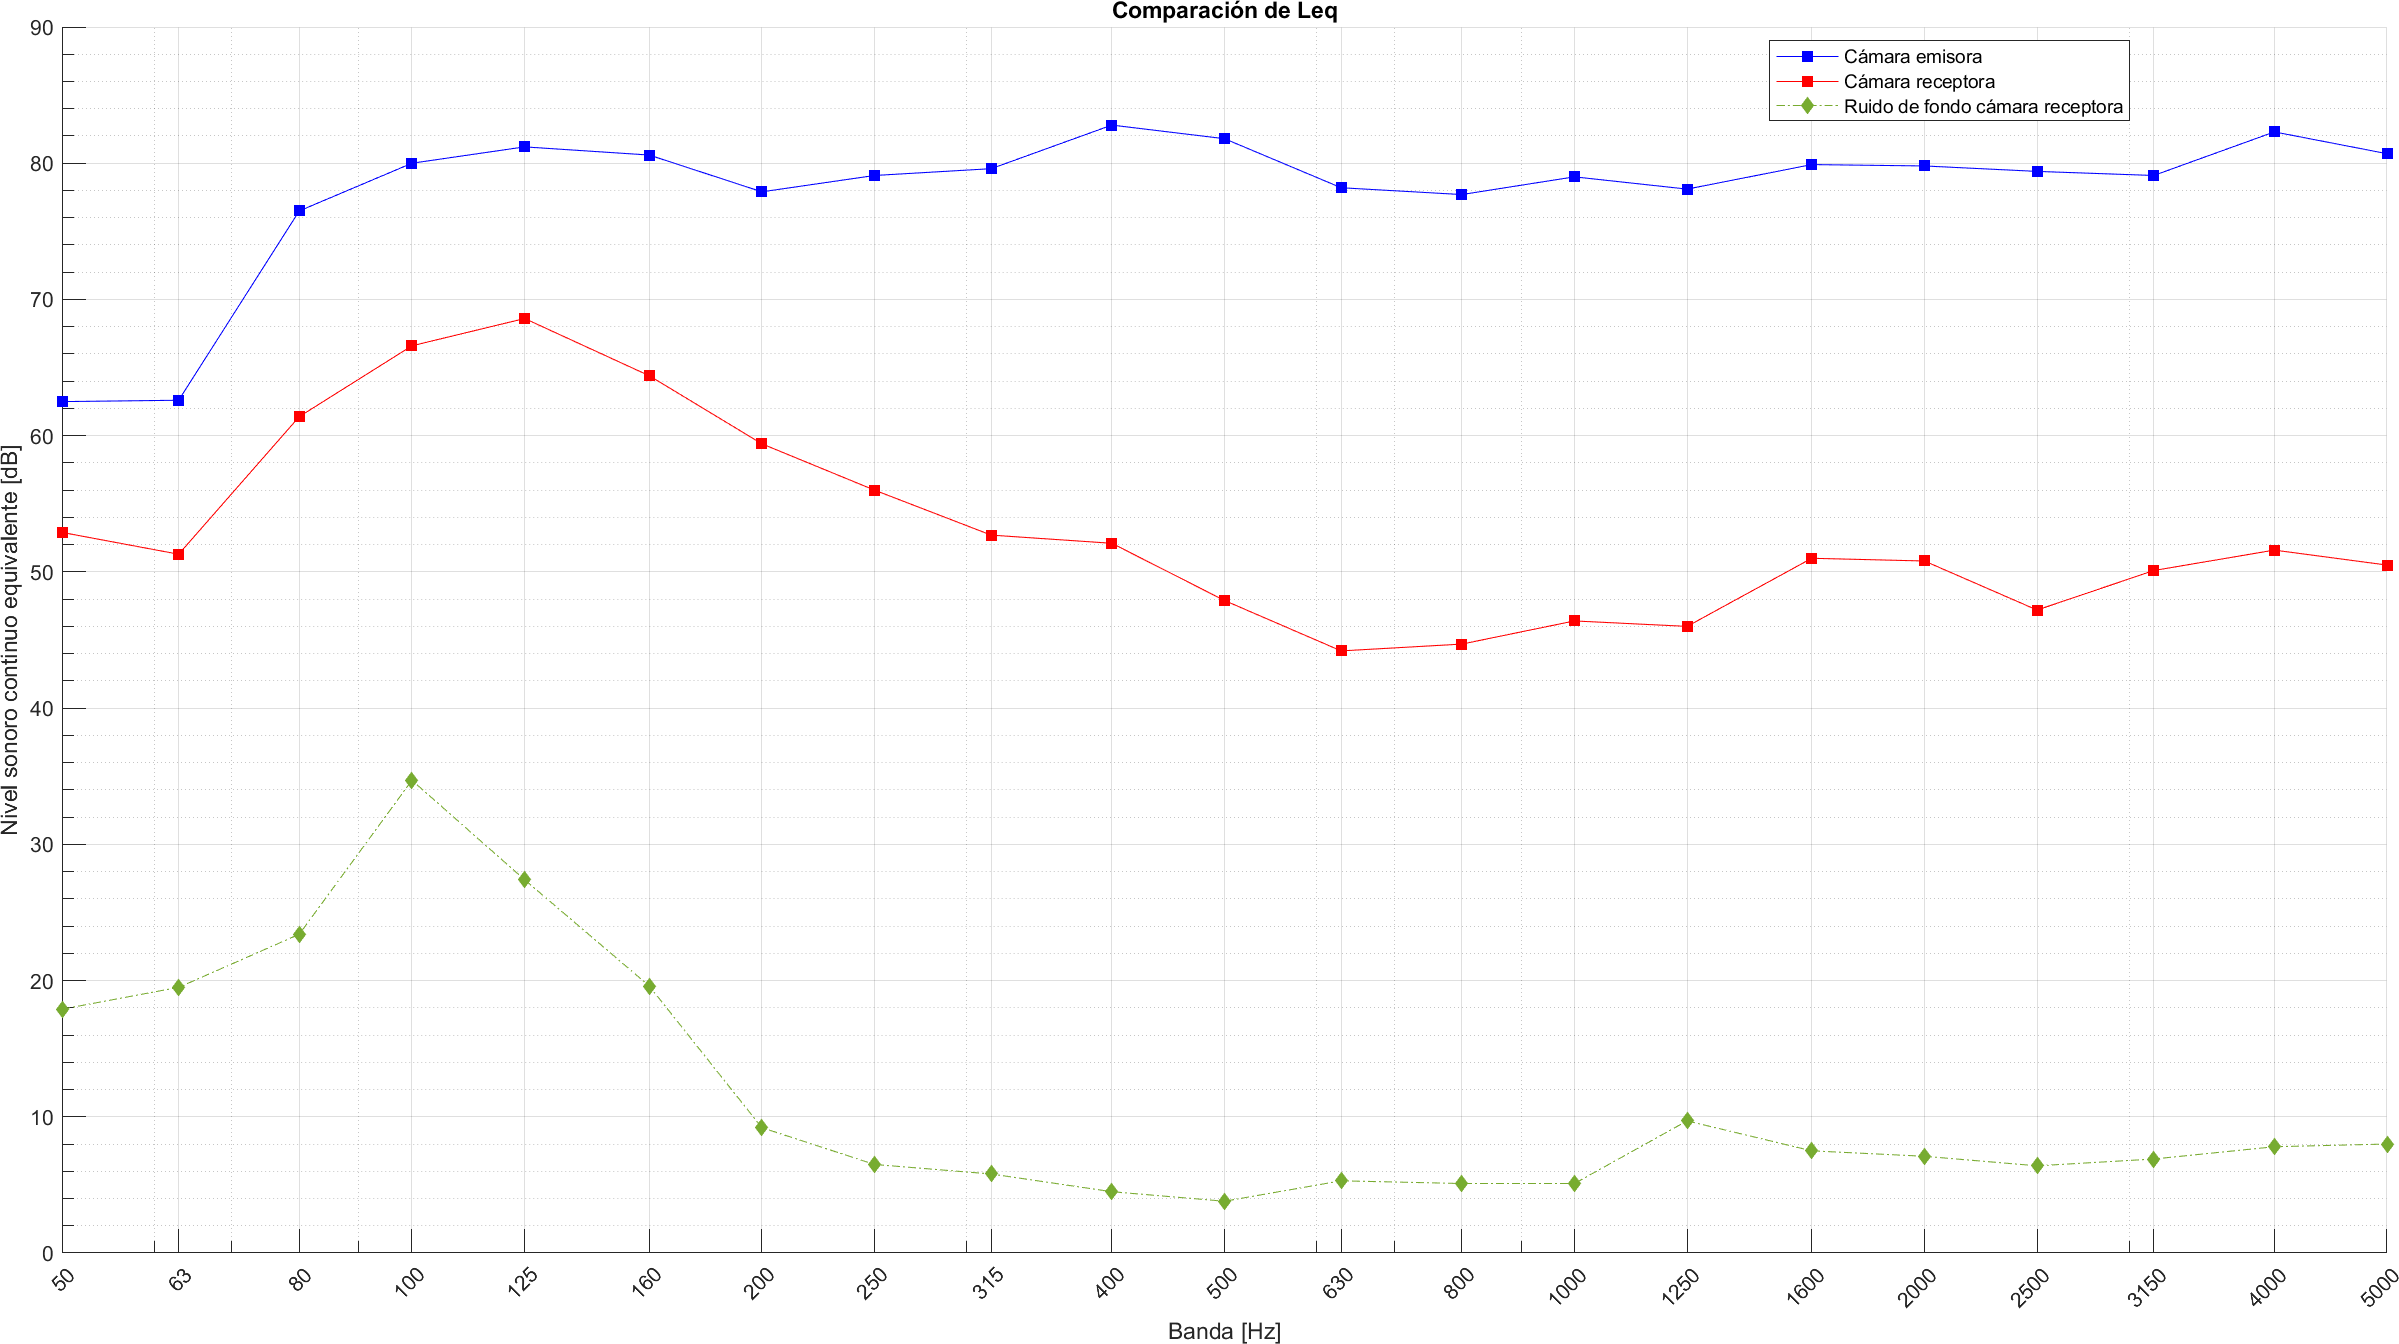
\includegraphics[width=0.98\textwidth]{./img/Comparacion_Leq.png}
%	\caption{Comparación de niveles sonoros medidos}
%	\label{fig::comparacion_niveles_sonoros}
%\end{figure}

\begin{figure}[H]
	\centering
	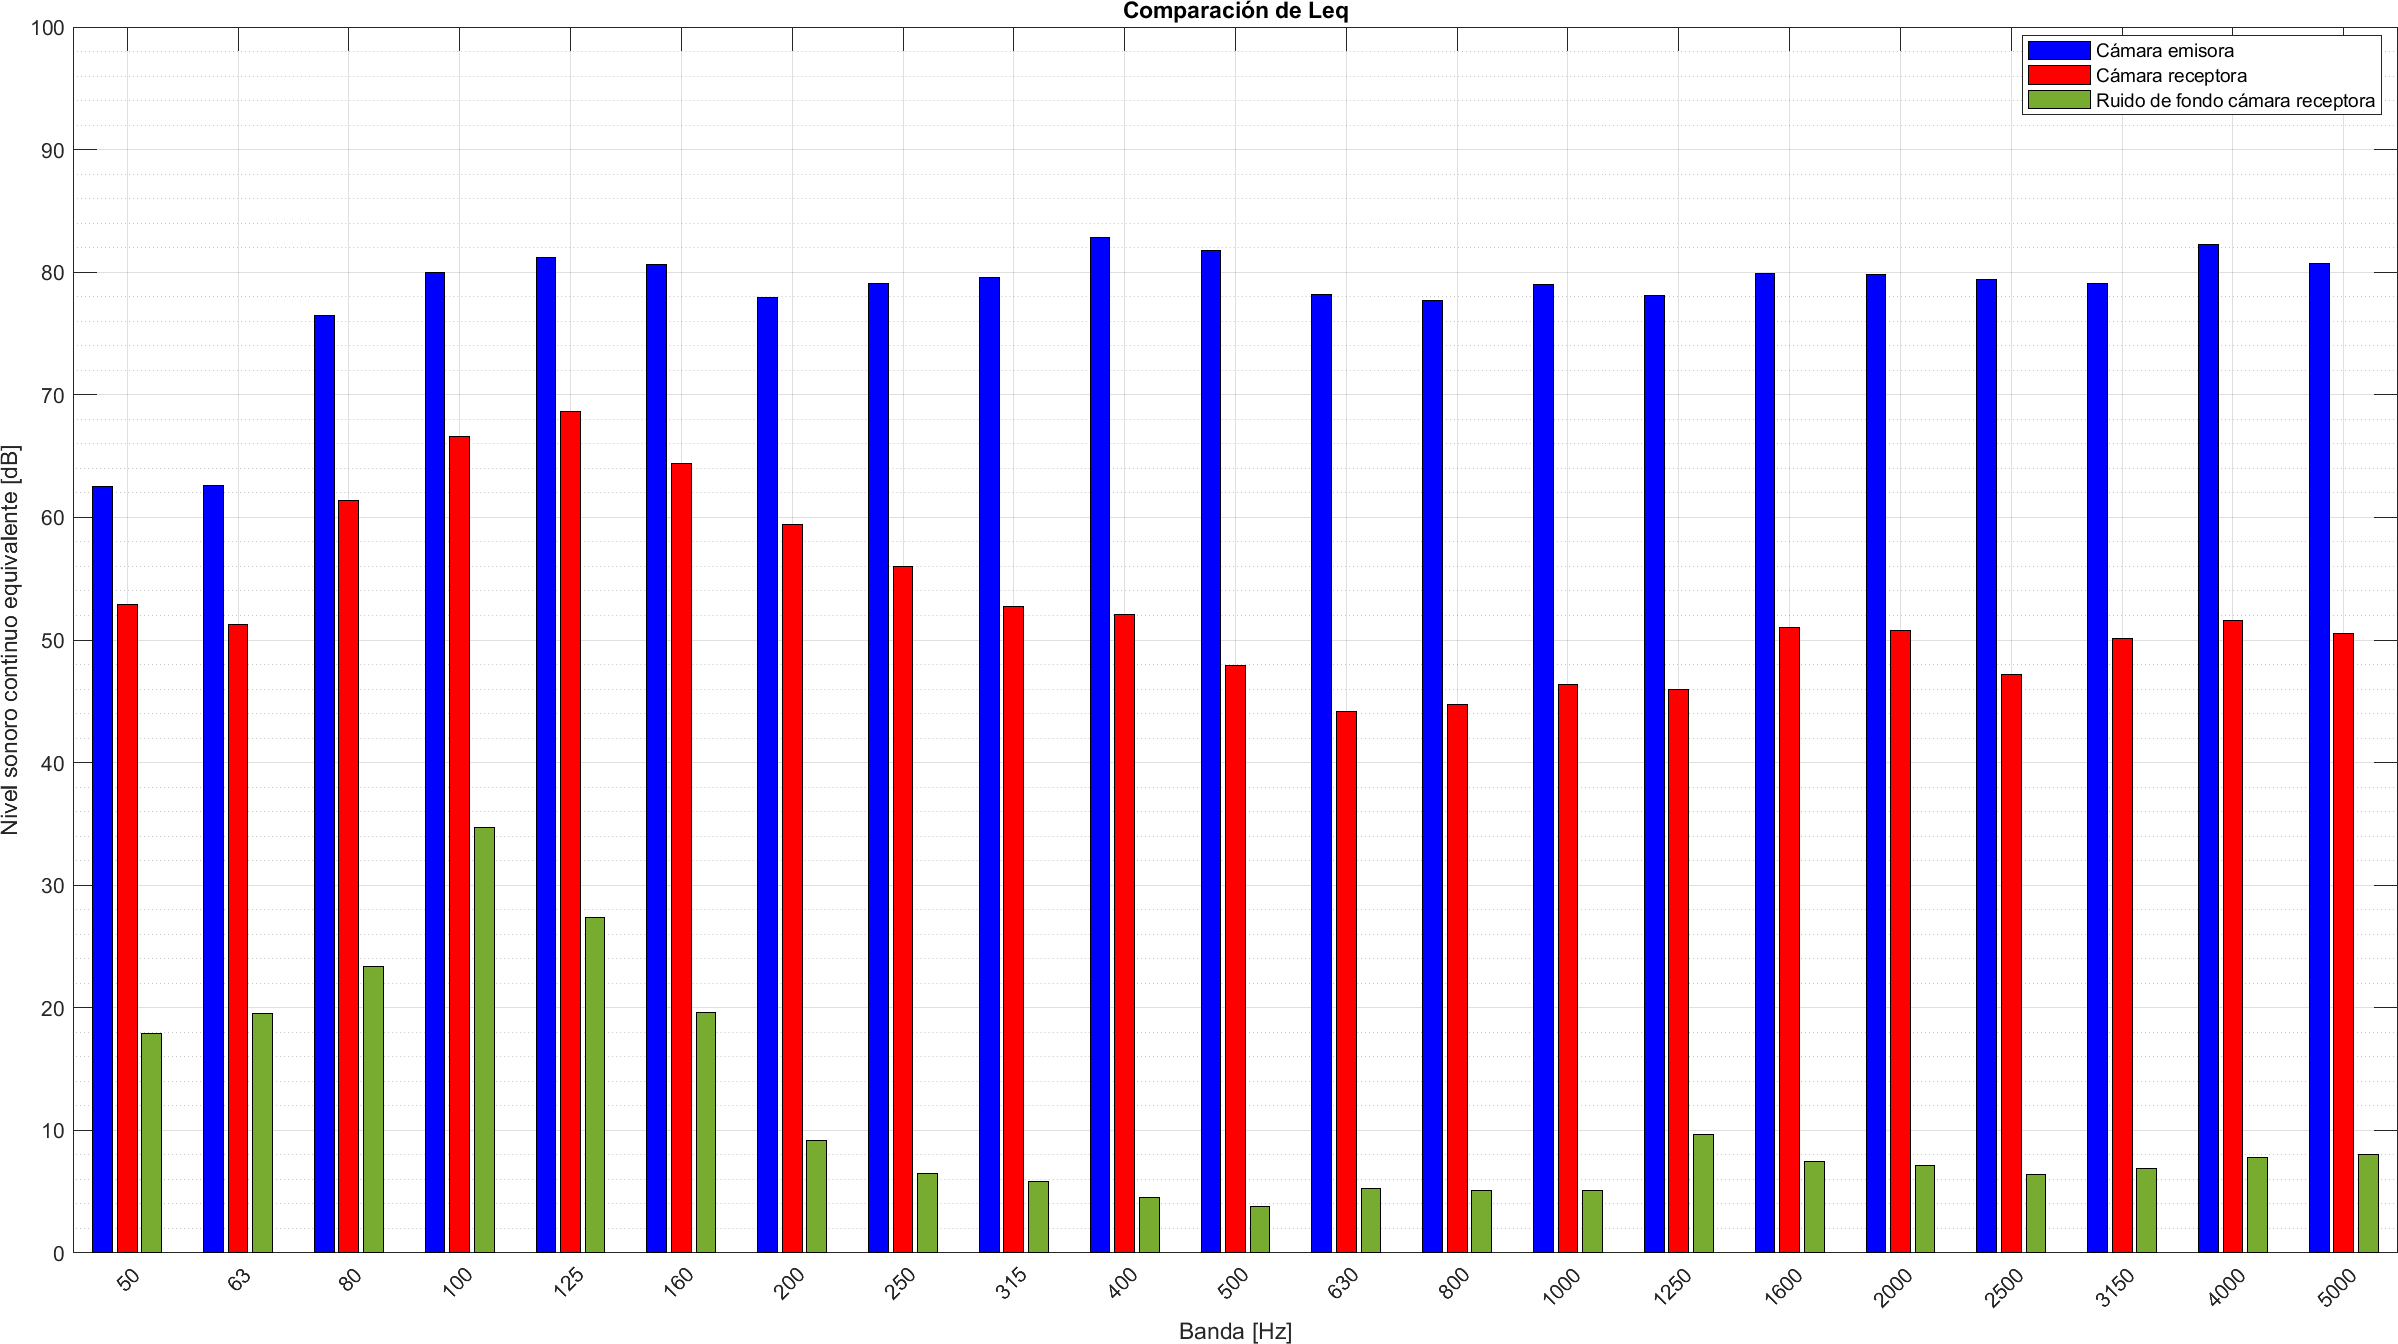
\includegraphics[width=0.98\textwidth]{./img/Comparacion_Leq_bars.png}
	\caption{Comparación de niveles sonoros medidos}
	\label{fig::comparacion_niveles_sonoros}
\end{figure}


\par En primer lugar, se observa con claridad una reducción en el nivel sonoro en la cámara receptora respecto a la emisora. Dicha diferencia, se hace más notable a frecuencias mayores, donde el material es más efectivo. Comienza por haber una diferencia de 10dB a bajas frecuencias y alcanza una diferencia máxima de 35dB. 


\par También puede observarse que los niveles sonoros del ruido de fondo de la cámara receptora, son muy bajos en comparación con los sonidos de prueba, mayores  a 25dB. Aún así se realiza la resta energética de los niveles medidos con el ruido de fondo para que este último no afecte en lo más mínimo con el análisis.\\

\par Una vez realizada dicha corrección, se calculan los valores de $R_i$ pertinentes, utilizando las ecuaciones mencionadas. Los resultados pueden observarse en el cuadro~ \tableref{tab:reduccion_sonora_R}, junto con el gráfico de la curva de $R$ en la figura~\figref{fig::indice_reduccion_sonora}.

%\begin{figure}[H]
%	\centering
%	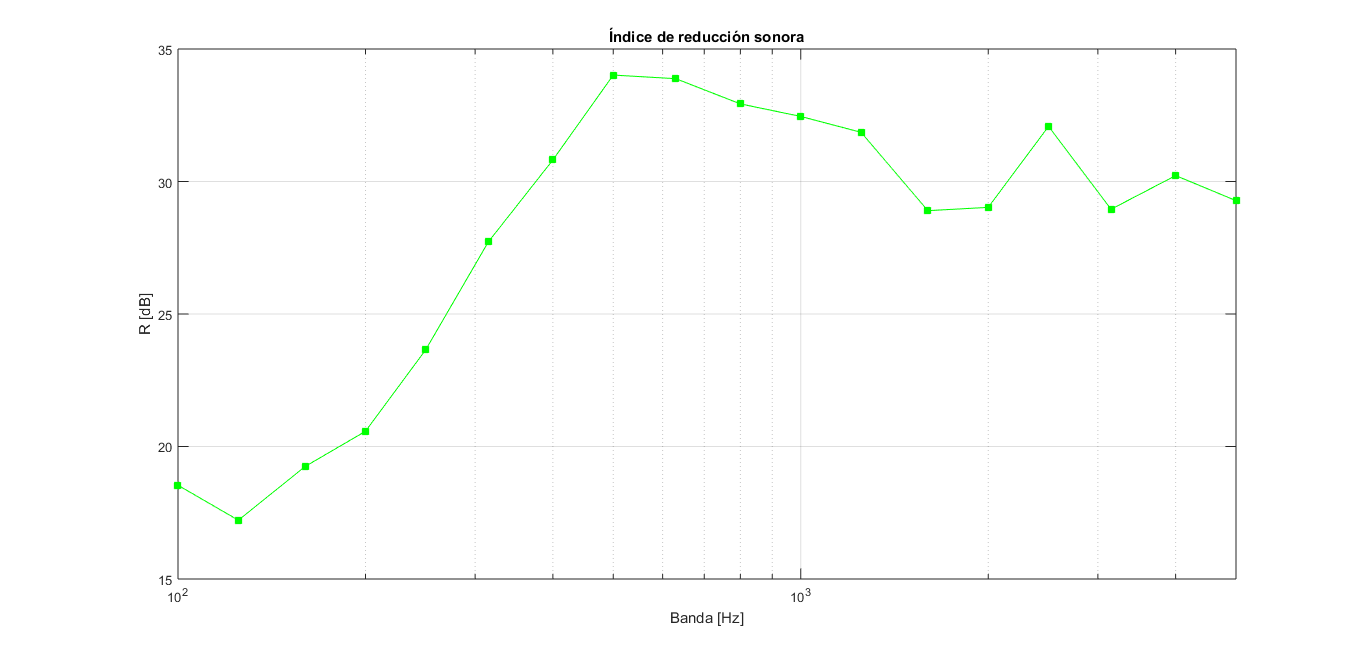
\includegraphics[width=0.98\textwidth]{./img/Indice_reduccion_sonora.png}
%	\caption{Curva de $R$}
%	\label{fig::indice_reduccion_sonora}
%\end{figure}


\begin{figure}[H]
	\centering
	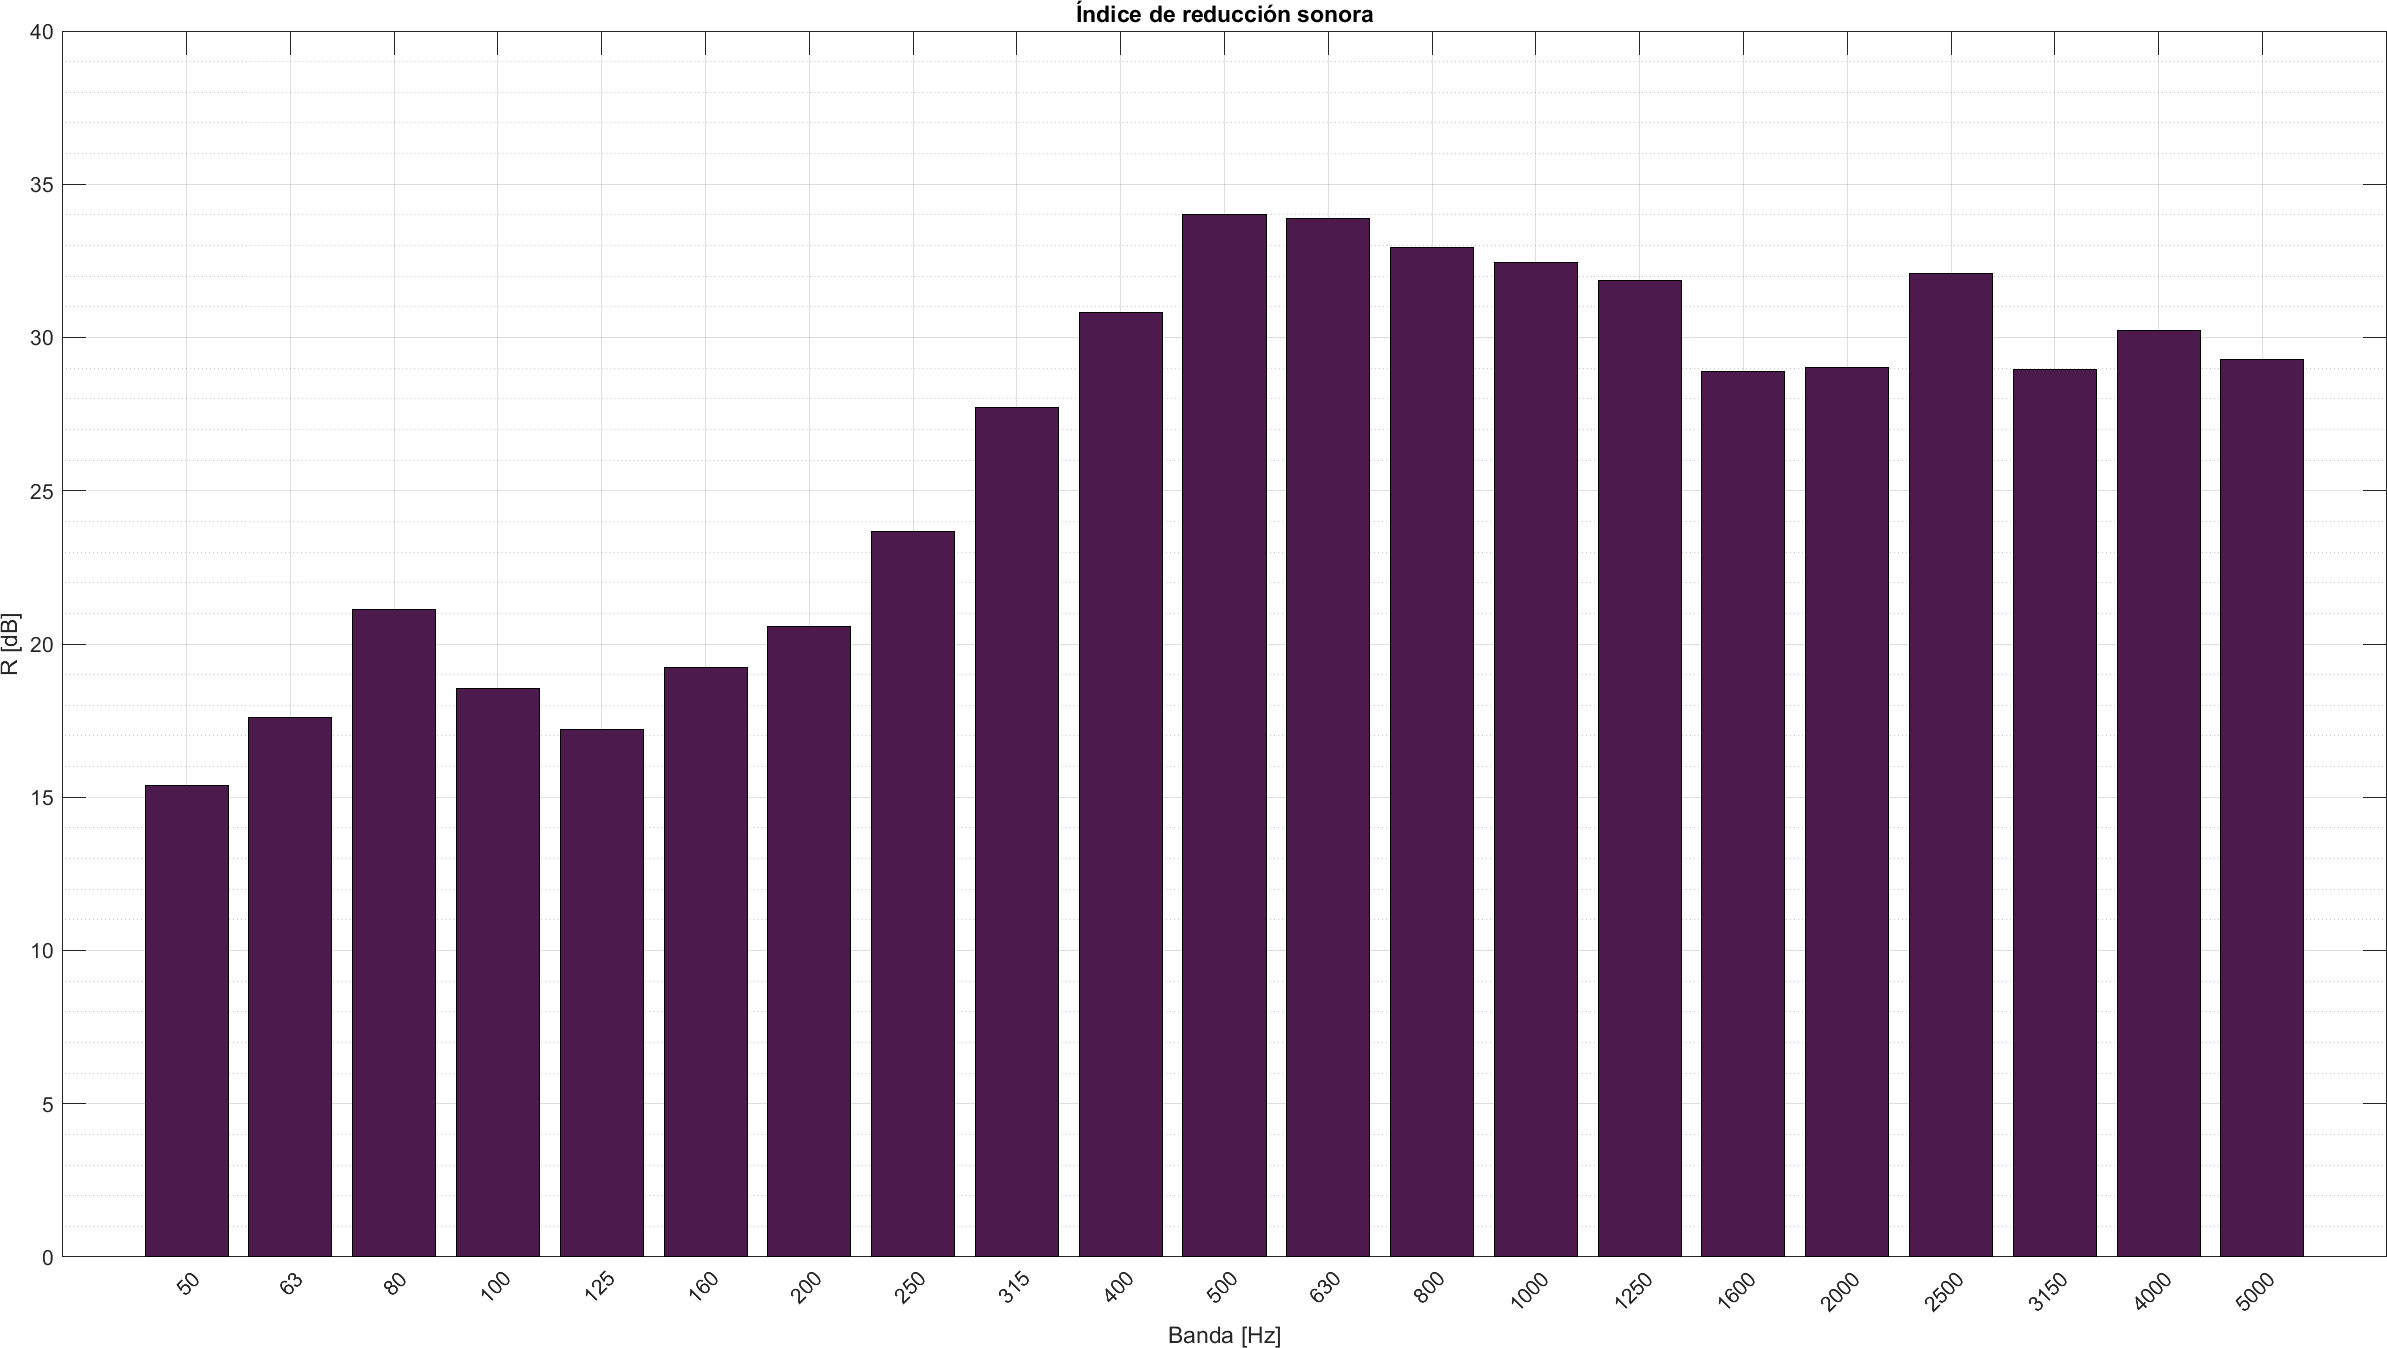
\includegraphics[width=0.98\textwidth]{./img/Indice_reduccion_sonora_bars.png}
	\caption{Curva de $R$}
	\label{fig::indice_reduccion_sonora}
\end{figure}


\par Como se observó en la Figura 1 y consecuentemente, era de esperarse en la Figura 2, existe una diferencia en la reducción sonora entre bajas y altas frecuencias. Alcanzando una diferencia máxima de $16dB$, y un valor máximo a los $50Hz$.

\par A partir de los datos de la Tabla~\tableref{tab:Niveles_sonoros_y_tiempos_de_reverberacion_medidos}, los valores de R obtenidos y de la ecuación~\eqref{eq:DL_R}, se obtiene el Índice de evaluación del aislamiento acústico:

\begin{equation*}
    DL_R =   29.5887 \approx 30
\end{equation*}

\par Para definir la categoría a la que pertenece la pantalla utilizada, es necesario conocer los valores de $DL_R$ asignados de acuerdo a la clasificación de la norma UNE-EN 1793-2:2014, Anexo A, presentados en el Cuadro 4. 

\begin{table}[H]
    \centering
    \begin{tabular}{|c|c|} \hline
        \textbf{Categoría} & \textbf{$DL_R$ en dB} \\ \hline \hline
         $B_0$ & No determinado \\ \hline
         $B_1$ & $DL_R < 15$  \\ \hline
         $B_2$ & 15 a 24 \\ \hline
         $B_3$ & 25 a 34 \\ \hline
         $B_4$ & $DL_R > 34$ \\ \hline
    \end{tabular}
    \caption{Categorías de comportamiento de aislamiento al ruido aéreo}
    \label{tab:categorias_aislamiento}
\end{table}


\par De forma concluyente en esta sección, podemos determinar que la pantalla diseñada  corresponde a la categoría $B_3$, como era deseado. Por ende, se determina válida su implementación en términos del aislamiento acústico buscado. 